% -------------------------------------------------------
% Pozostałe wykresy benchmarków (scenariusze nieomówione w sekcji głównej)
% -------------------------------------------------------

\subsection{Wolumen small - 500 000 rekordów}

% -------------------------------------------------------
% INSERT
% -------------------------------------------------------

\subsubsection{I1: Rejestracja użytkownika}
\begin{figure}[H]
    \centering
    
\includegraphics[width=0.8\textwidth]{charts/small/chart_I1.png}
    \caption{I1 -- Rejestracja użytkownika (small)}
\end{figure}

\subsubsection{I4: Batch insert płatności}
\begin{figure}[H]
    \centering
    
\includegraphics[width=0.8\textwidth]{charts/small/chart_I4.png}
    \caption{I4 -- Batch insert płatności (small)}
\end{figure}

\subsubsection{I5: Oceny z przeliczeniem średniej}
\begin{figure}[H]
    \centering
    
\includegraphics[width=0.8\textwidth]{charts/small/chart_I5.png}
    \caption{I5 -- Oceny z przeliczeniem średniej oceny (small)}
\end{figure}

\subsubsection{I6: Import osób z powiązaniami}
\begin{figure}[H]
    \centering
    
\includegraphics[width=0.8\textwidth]{charts/small/chart_I6.png}
    \caption{I6 -- Import osób z powiązaniami (small)}
\end{figure}

% -------------------------------------------------------
% SELECT
% -------------------------------------------------------

\subsubsection{S1: Strona główna}
\begin{figure}[H]
    \centering
    
\includegraphics[width=0.8\textwidth]{charts/small/chart_S1.png}
    \caption{S1 -- Strona główna (small)}
\end{figure}

\subsubsection{S5: Historia oglądania profilu}
\begin{figure}[H]
    \centering
    
\includegraphics[width=0.8\textwidth]{charts/small/chart_S5.png}
    \caption{S5 -- Historia oglądania profilu (small)}
\end{figure}

\subsubsection{S6: Filmografia osoby}
\begin{figure}[H]
    \centering
    
\includegraphics[width=0.8\textwidth]{charts/small/chart_S6.png}
    \caption{S6 -- Filmografia osoby (small)}
\end{figure}

% -------------------------------------------------------
% DELETE
% -------------------------------------------------------

\subsubsection{D2: Usunięcie profilu z historią}
\begin{figure}[H]
    \centering
    
\includegraphics[width=0.8\textwidth]{charts/small/chart_D2.png}
    \caption{D2 -- Usunięcie profilu z historią (small)}
\end{figure}

\subsubsection{D3: Czyszczenie starych ocen}
\begin{figure}[H]
    \centering
    
\includegraphics[width=0.8\textwidth]{charts/small/chart_D3.png}
    \caption{D3 -- Czyszczenie starych ocen (small)}
\end{figure}

\subsubsection{D5: Usunięcie subskrypcji z płatnościami}
\begin{figure}[H]
    \centering
    
\includegraphics[width=0.8\textwidth]{charts/small/chart_D5.png}
    \caption{D5 -- Usunięcie subskrypcji z płatnościami (small)}
\end{figure}

% -------------------------------------------------------
% UPDATE
% -------------------------------------------------------

\subsubsection{U1: Aktualizacja postępu oglądania}
\begin{figure}[H]
    \centering
    
\includegraphics[width=0.8\textwidth]{charts/small/chart_U1.png}
    \caption{U1 -- Aktualizacja postępu oglądania (small)}
\end{figure}

\subsubsection{U4: Aktualizacja danych użytkownika}
\begin{figure}[H]
    \centering
    
\includegraphics[width=0.8\textwidth]{charts/small/chart_U4.png}
    \caption{U4 -- Aktualizacja danych użytkownika (small)}
\end{figure}

\subsubsection{U5: Oznaczenie treści jako nieaktywnej}
\begin{figure}[H]
    \centering
    
\includegraphics[width=0.8\textwidth]{charts/small/chart_U5.png}
    \caption{U5 -- Oznaczenie treści jako nieaktywnej (small)}
\end{figure}

\subsubsection{U6: Masowa aktualizacja wskaźnika popularności}
\begin{figure}[H]
    \centering
    
\includegraphics[width=0.8\textwidth]{charts/small/chart_U6.png}
    \caption{U6 -- Masowa aktualizacja wskaźnika popularności (small)}
\end{figure}


\subsection{Wolumen medium - 1 000 000 rekordów}

% -------------------------------------------------------
% INSERT
% -------------------------------------------------------

\subsubsection{I1: Rejestracja użytkownika}
\begin{figure}[H]
    \centering
    
\includegraphics[width=0.8\textwidth]{charts/medium/chart_I1.png}
    \caption{I1 -- Rejestracja użytkownika (medium)}
\end{figure}

\subsubsection{I4: Batch insert płatności}
\begin{figure}[H]
    \centering
    
\includegraphics[width=0.8\textwidth]{charts/medium/chart_I4.png}
    \caption{I4 -- Batch insert płatności (medium)}
\end{figure}

\subsubsection{I5: Oceny z przeliczeniem średniej}
\begin{figure}[H]
    \centering
    
\includegraphics[width=0.8\textwidth]{charts/medium/chart_I5.png}
    \caption{I5 -- Oceny z przeliczeniem średniej oceny (medium)}
\end{figure}

\subsubsection{I6: Import osób z powiązaniami}
\begin{figure}[H]
    \centering
    
\includegraphics[width=0.8\textwidth]{charts/medium/chart_I6.png}
    \caption{I6 -- Import osób z powiązaniami (medium)}
\end{figure}

% -------------------------------------------------------
% SELECT
% -------------------------------------------------------

\subsubsection{S1: Strona główna}
\begin{figure}[H]
    \centering
    
\includegraphics[width=0.8\textwidth]{charts/medium/chart_S1.png}
    \caption{S1 -- Strona główna (medium)}
\end{figure}

\subsubsection{S5: Historia oglądania profilu}
\begin{figure}[H]
    \centering
    
\includegraphics[width=0.8\textwidth]{charts/medium/chart_S5.png}
    \caption{S5 -- Historia oglądania profilu (medium)}
\end{figure}

\subsubsection{S6: Filmografia osoby}
\begin{figure}[H]
    \centering
    
\includegraphics[width=0.8\textwidth]{charts/medium/chart_S6.png}
    \caption{S6 -- Filmografia osoby (medium)}
\end{figure}

% -------------------------------------------------------
% DELETE
% -------------------------------------------------------

\subsubsection{D2: Usunięcie profilu z historią}
\begin{figure}[H]
    \centering
    
\includegraphics[width=0.8\textwidth]{charts/medium/chart_D2.png}
    \caption{D2 -- Usunięcie profilu z historią (medium)}
\end{figure}

\subsubsection{D3: Czyszczenie starych ocen}
\begin{figure}[H]
    \centering
    
\includegraphics[width=0.8\textwidth]{charts/medium/chart_D3.png}
    \caption{D3 -- Czyszczenie starych ocen (medium)}
\end{figure}

\subsubsection{D5: Usunięcie subskrypcji z płatnościami}
\begin{figure}[H]
    \centering
    
\includegraphics[width=0.8\textwidth]{charts/medium/chart_D5.png}
    \caption{D5 -- Usunięcie subskrypcji z płatnościami (medium)}
\end{figure}

% -------------------------------------------------------
% UPDATE
% -------------------------------------------------------

\subsubsection{U1: Aktualizacja postępu oglądania}
\begin{figure}[H]
    \centering
    
\includegraphics[width=0.8\textwidth]{charts/medium/chart_U1.png}
    \caption{U1 -- Aktualizacja postępu oglądania (medium)}
\end{figure}

\subsubsection{U4: Aktualizacja danych użytkownika}
\begin{figure}[H]
    \centering
    
\includegraphics[width=0.8\textwidth]{charts/medium/chart_U4.png}
    \caption{U4 -- Aktualizacja danych użytkownika (medium)}
\end{figure}

\subsubsection{U5: Oznaczenie treści jako nieaktywnej}
\begin{figure}[H]
    \centering
    
\includegraphics[width=0.8\textwidth]{charts/medium/chart_U5.png}
    \caption{U5 -- Oznaczenie treści jako nieaktywnej (medium)}
\end{figure}

\subsubsection{U6: Masowa aktualizacja wskaźnika popularności}
\begin{figure}[H]
    \centering
    
\includegraphics[width=0.8\textwidth]{charts/medium/chart_U6.png}
    \caption{U6 -- Masowa aktualizacja wskaźnika popularności (medium)}
\end{figure}


\subsection{Wolumen large - 10 000 000 rekordów}

% -------------------------------------------------------
% INSERT
% -------------------------------------------------------

\subsubsection{I1: Rejestracja użytkownika}
\begin{figure}[H]
    \centering
    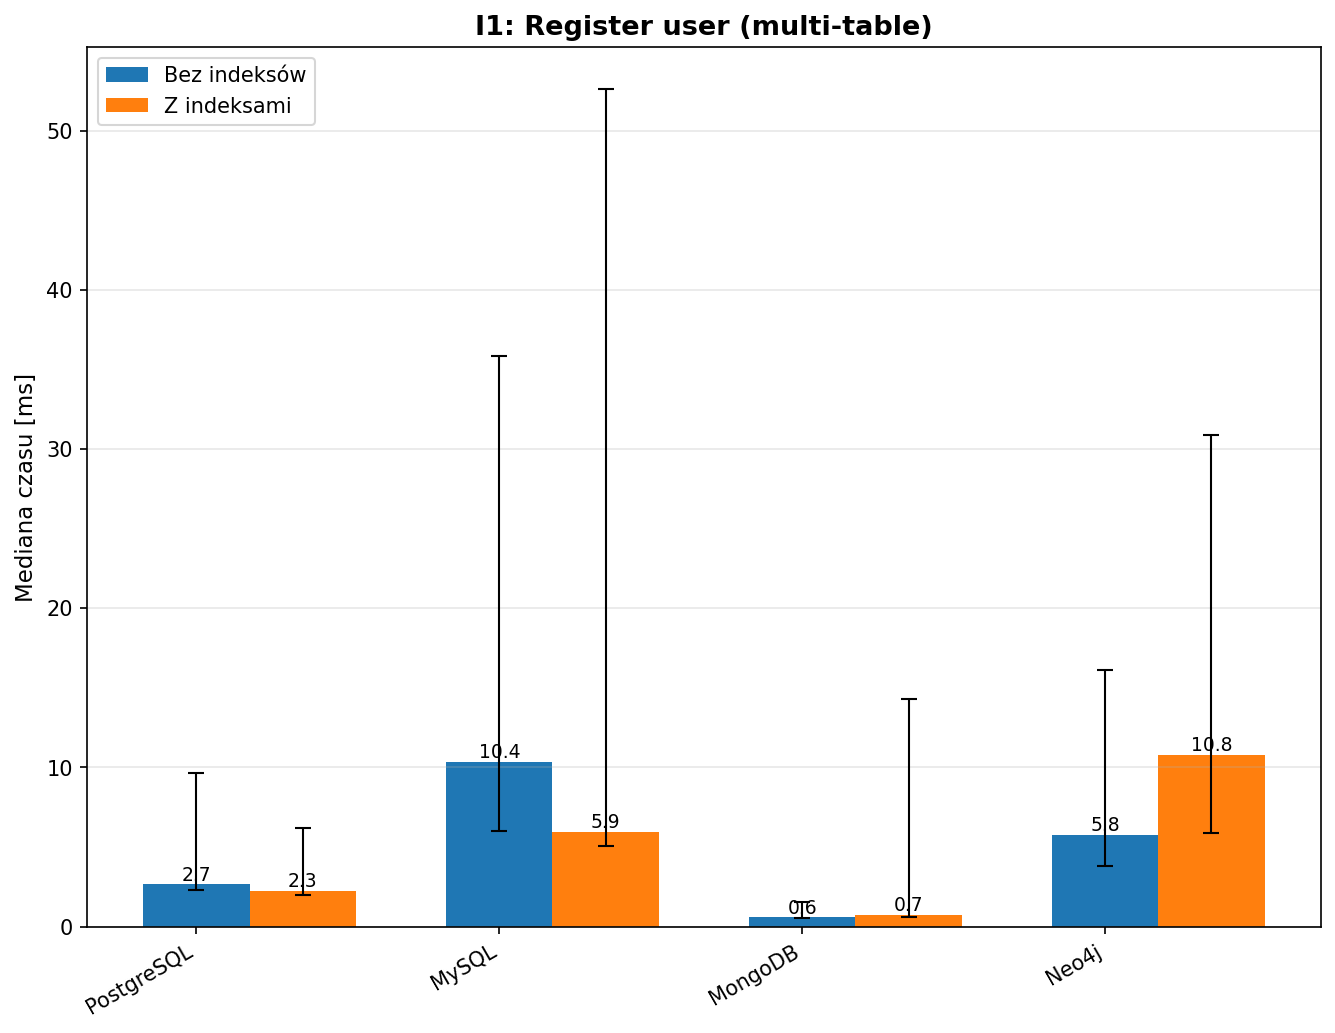
\includegraphics[width=0.8\textwidth]{charts/large/chart_I1.png}
    \caption{I1 -- Rejestracja użytkownika (large)}
\end{figure}

\subsubsection{I4: Batch insert płatności}
\begin{figure}[H]
    \centering
    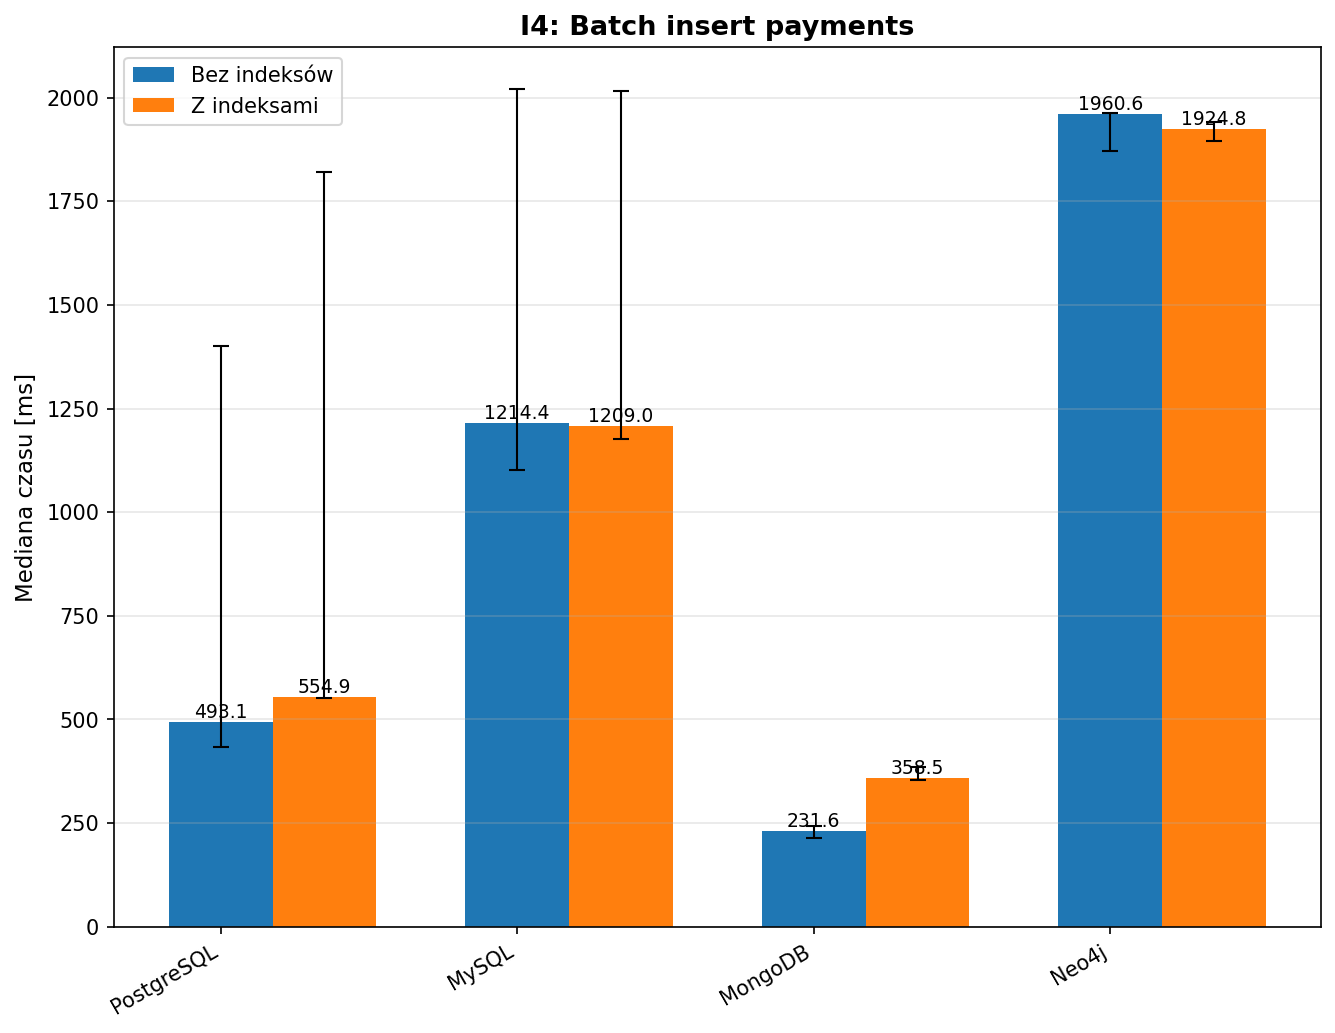
\includegraphics[width=0.8\textwidth]{charts/large/chart_I4.png}
    \caption{I4 -- Batch insert płatności (large)}
\end{figure}

\subsubsection{I5: Oceny z przeliczeniem średniej}
\begin{figure}[H]
    \centering
    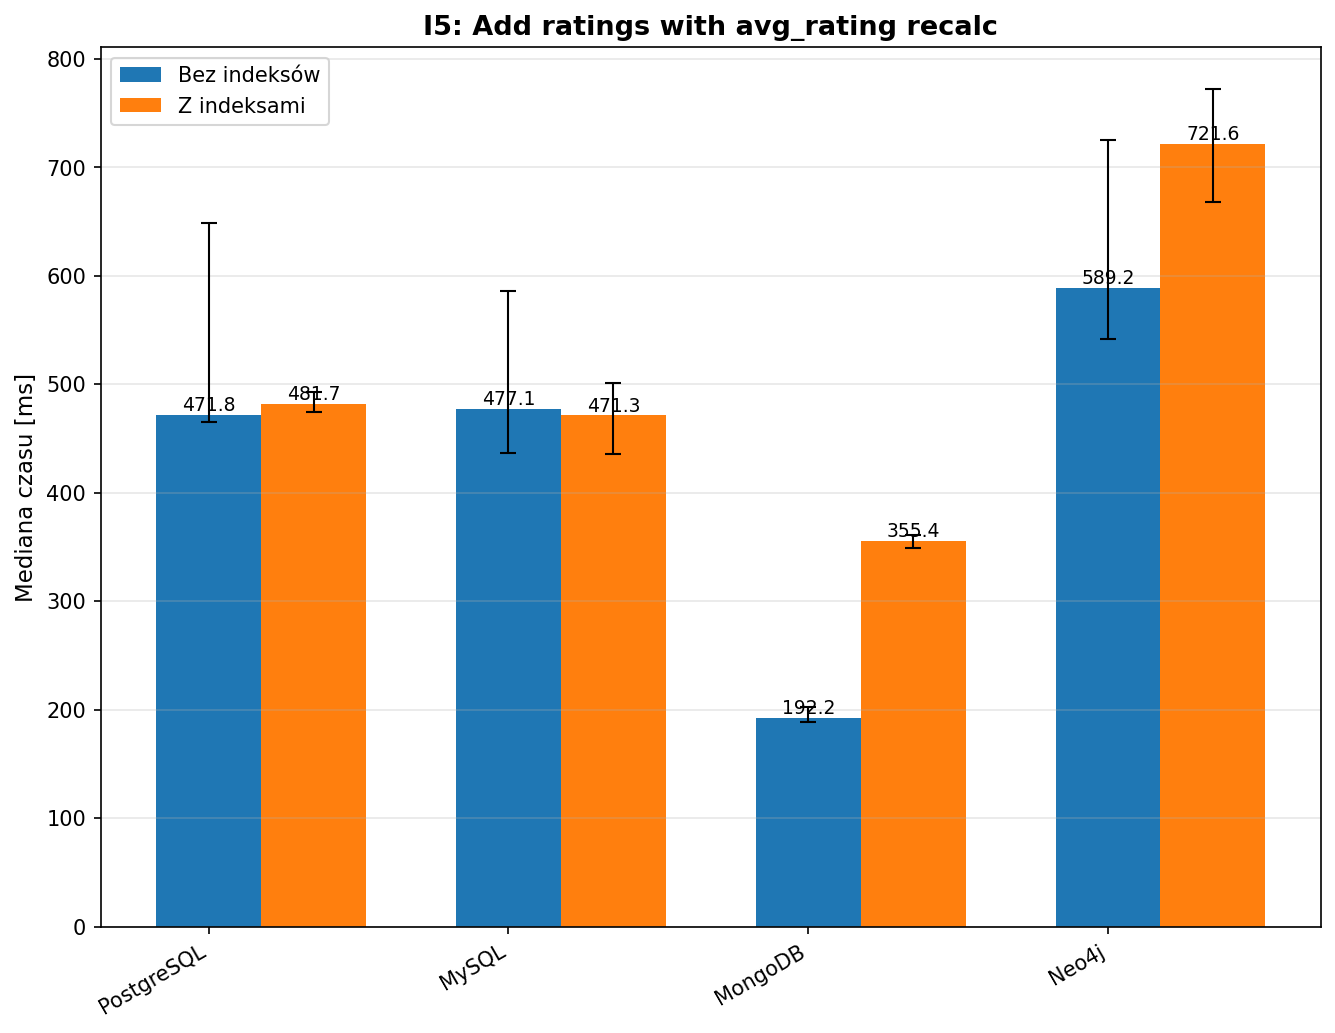
\includegraphics[width=0.8\textwidth]{charts/large/chart_I5.png}
    \caption{I5 -- Oceny z przeliczeniem średniej oceny (large)}
\end{figure}

\subsubsection{I6: Import osób z powiązaniami}
\begin{figure}[H]
    \centering
    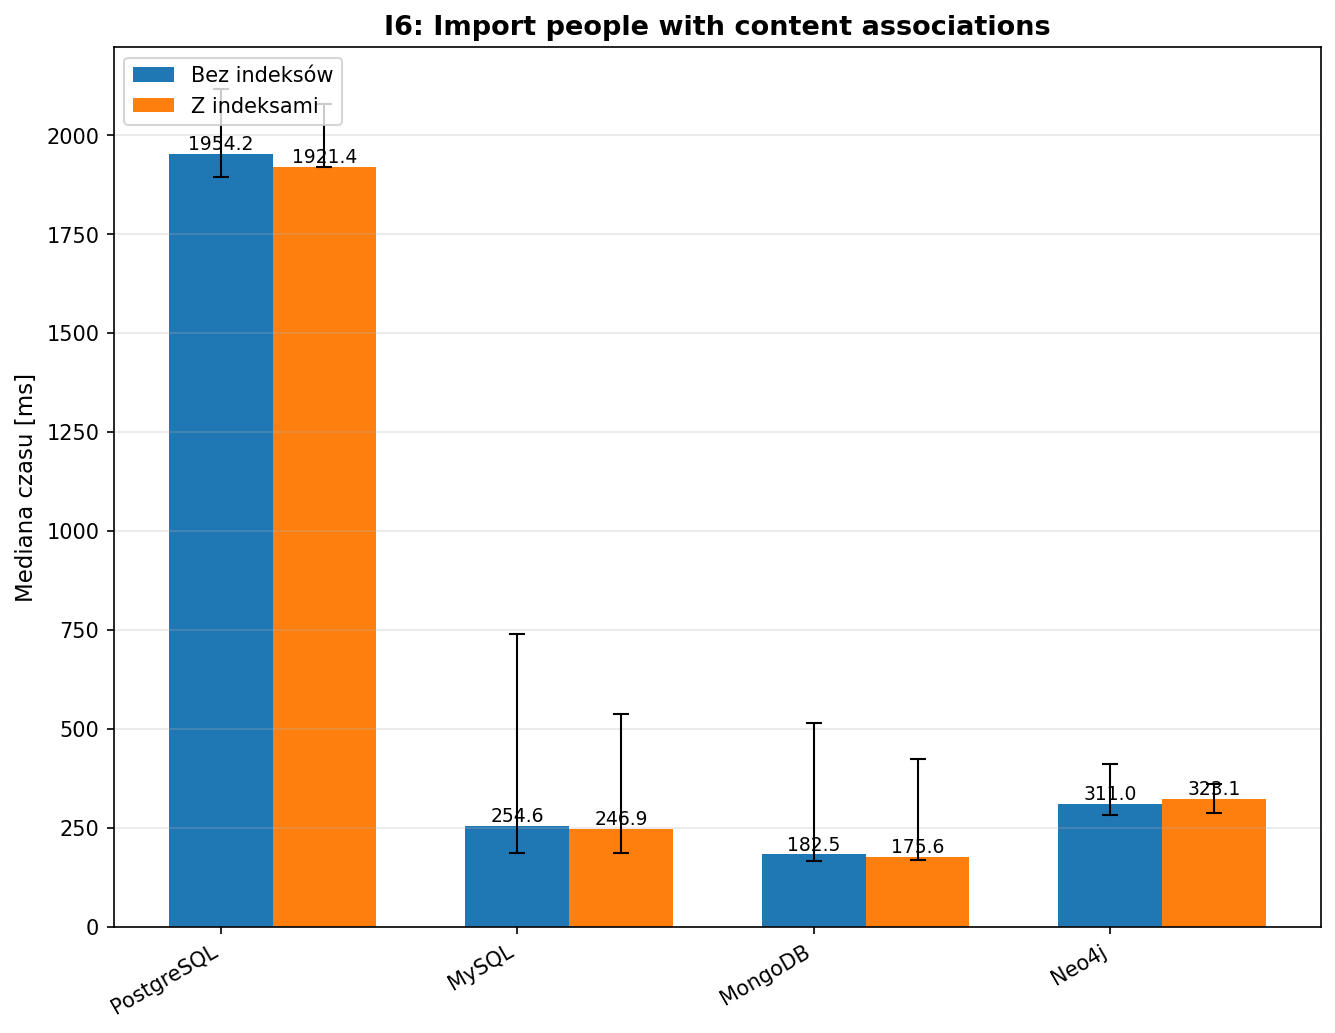
\includegraphics[width=0.8\textwidth]{charts/large/chart_I6.png}
    \caption{I6 -- Import osób z powiązaniami (large)}
\end{figure}

% -------------------------------------------------------
% SELECT
% -------------------------------------------------------

\subsubsection{S1: Strona główna}
\begin{figure}[H]
    \centering
    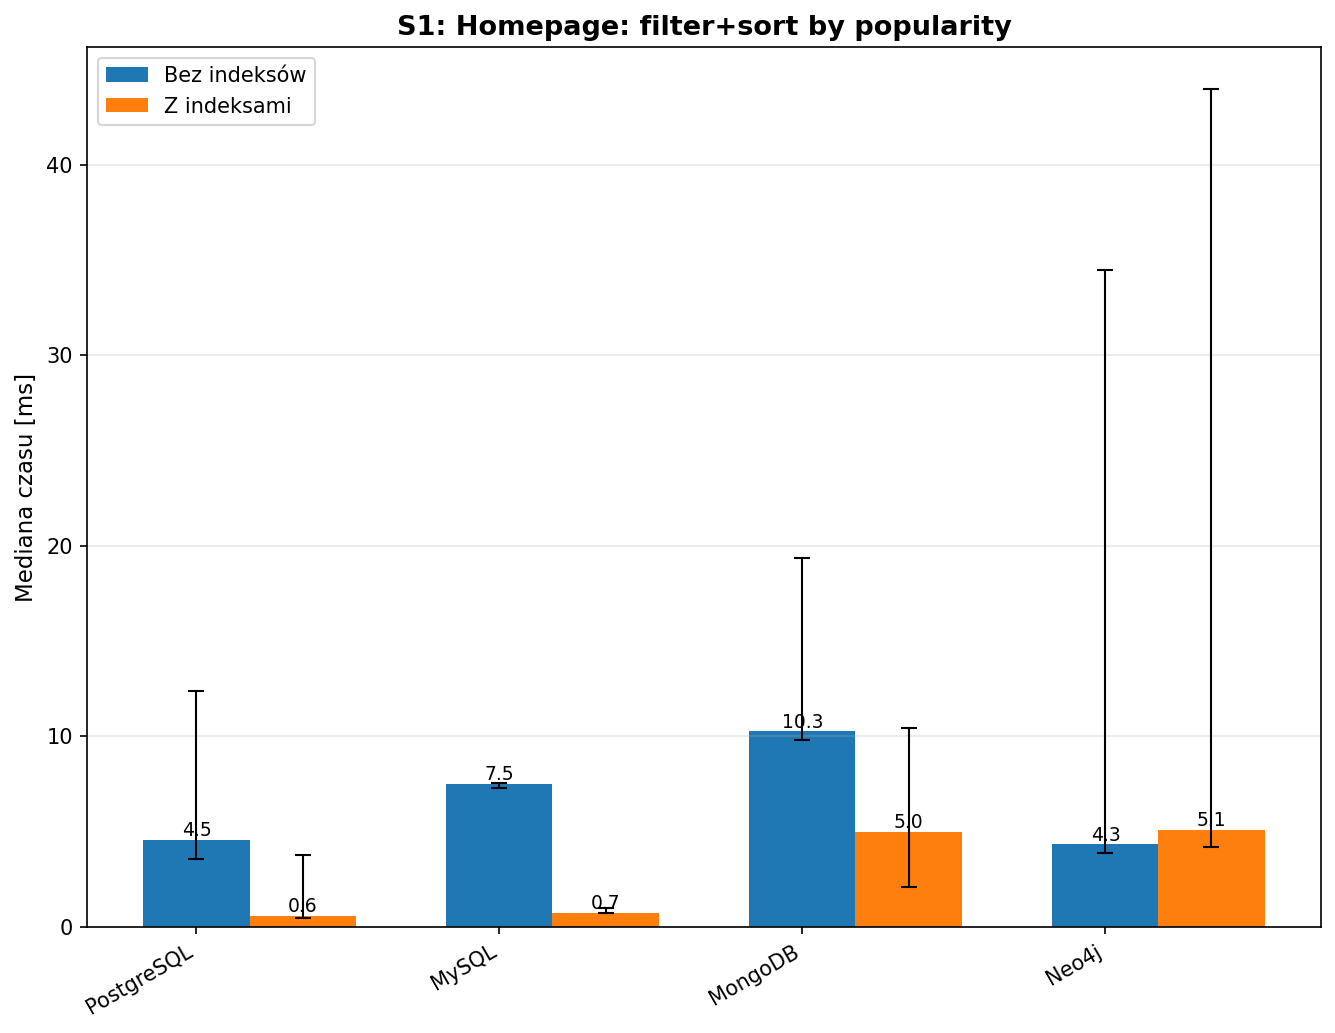
\includegraphics[width=0.8\textwidth]{charts/large/chart_S1.png}
    \caption{S1 -- Strona główna (large)}
\end{figure}

\subsubsection{S5: Historia oglądania profilu}
\begin{figure}[H]
    \centering
    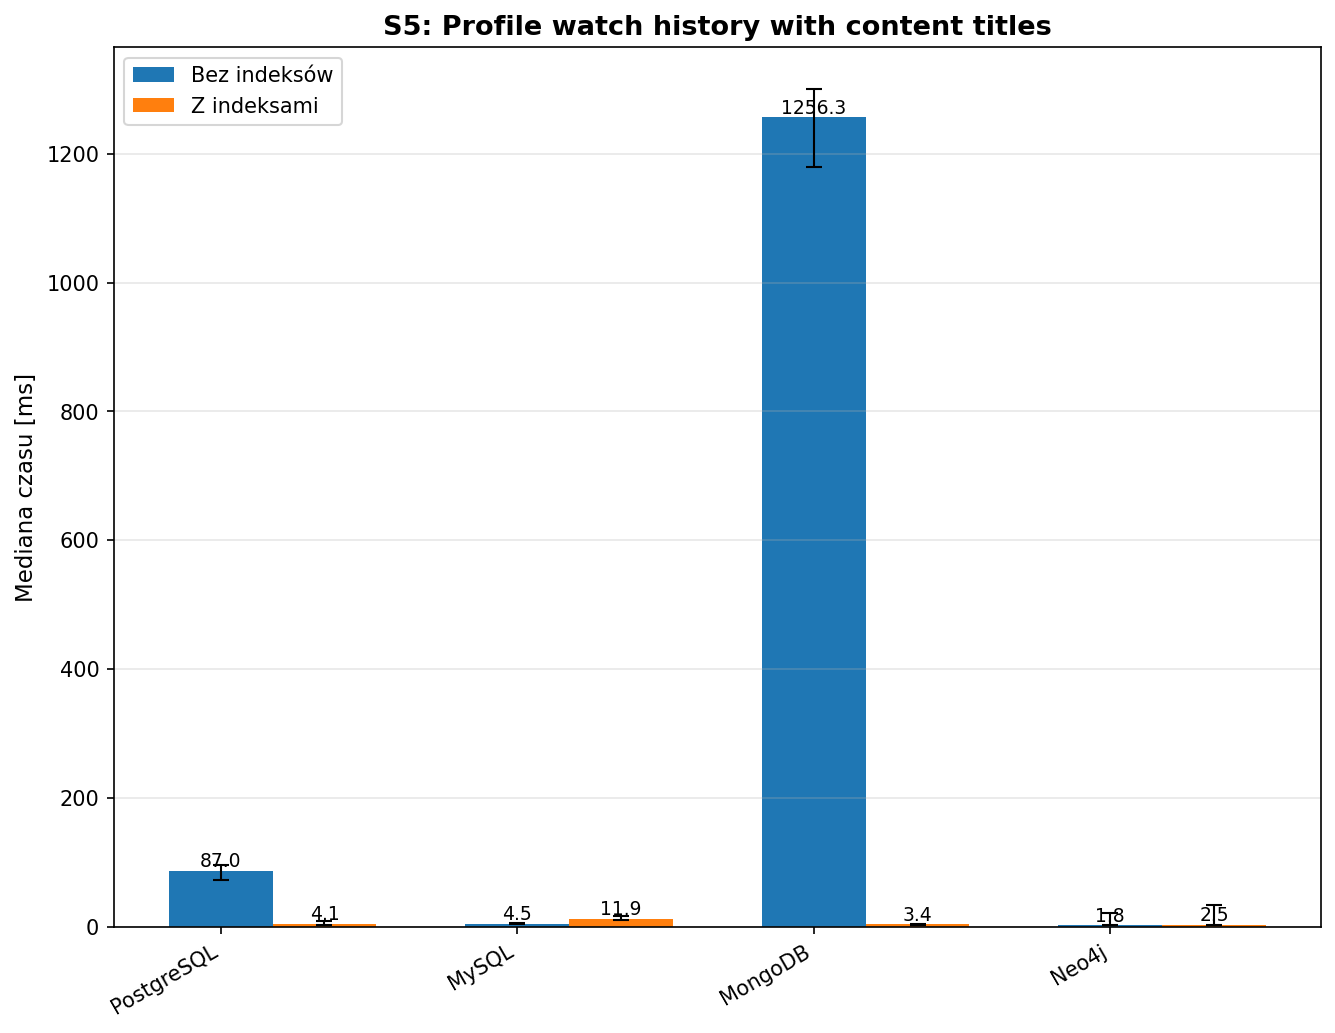
\includegraphics[width=0.8\textwidth]{charts/large/chart_S5.png}
    \caption{S5 -- Historia oglądania profilu (large)}
\end{figure}

\subsubsection{S6: Filmografia osoby}
\begin{figure}[H]
    \centering
    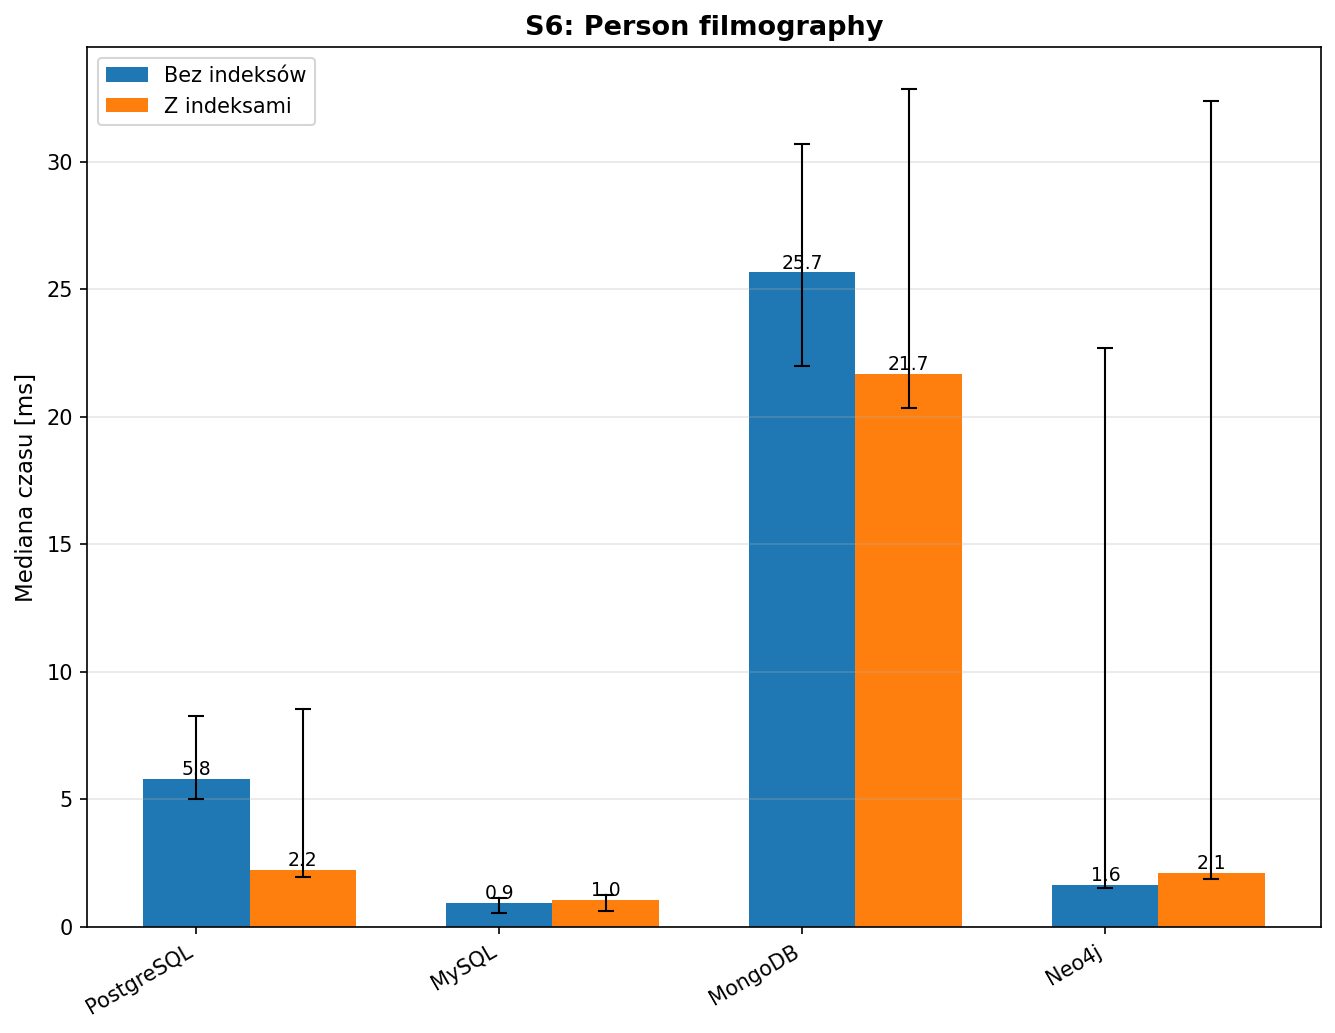
\includegraphics[width=0.8\textwidth]{charts/large/chart_S6.png}
    \caption{S6 -- Filmografia osoby (large)}
\end{figure}

% -------------------------------------------------------
% DELETE
% -------------------------------------------------------

\subsubsection{D2: Usunięcie profilu z historią}
\begin{figure}[H]
    \centering
    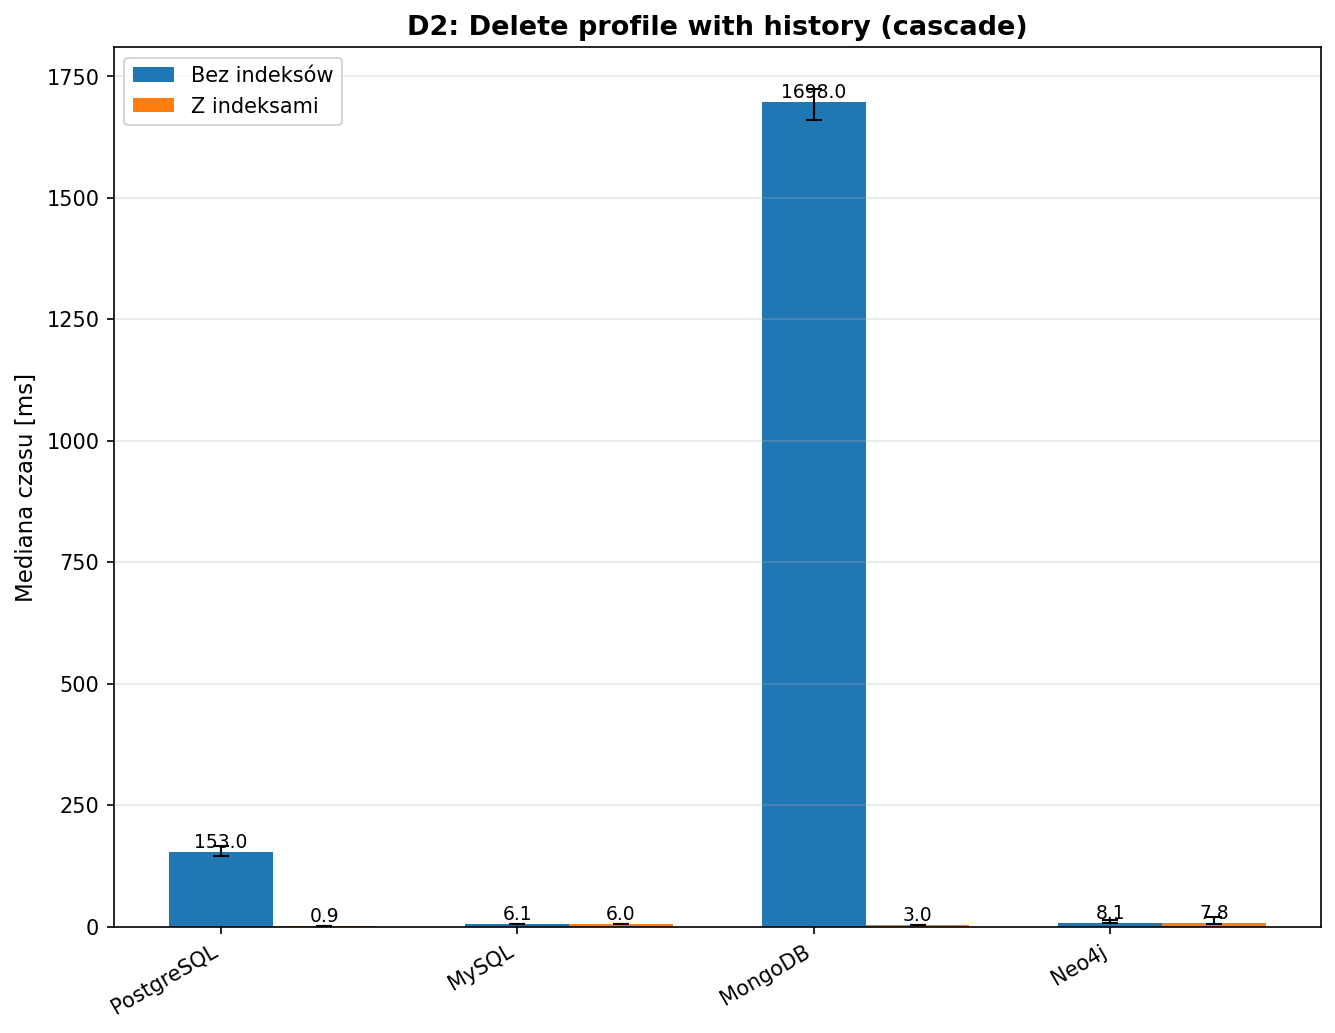
\includegraphics[width=0.8\textwidth]{charts/large/chart_D2.png}
    \caption{D2 -- Usunięcie profilu z historią (large)}
\end{figure}

\subsubsection{D3: Czyszczenie starych ocen}
\begin{figure}[H]
    \centering
    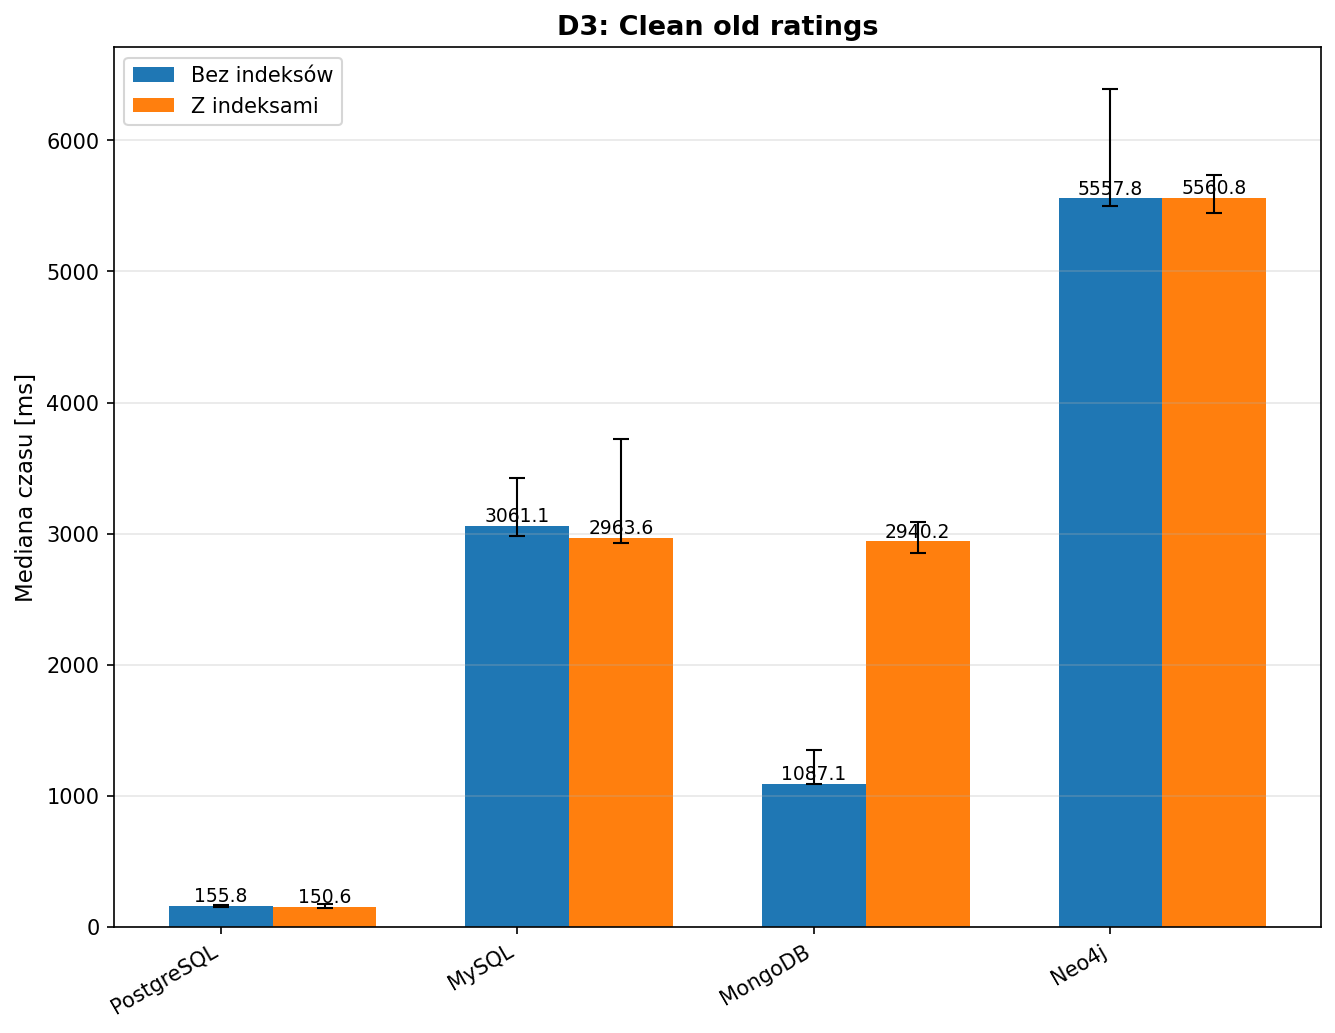
\includegraphics[width=0.8\textwidth]{charts/large/chart_D3.png}
    \caption{D3 -- Czyszczenie starych ocen (large)}
\end{figure}

\subsubsection{D5: Usunięcie subskrypcji z płatnościami}
\begin{figure}[H]
    \centering
    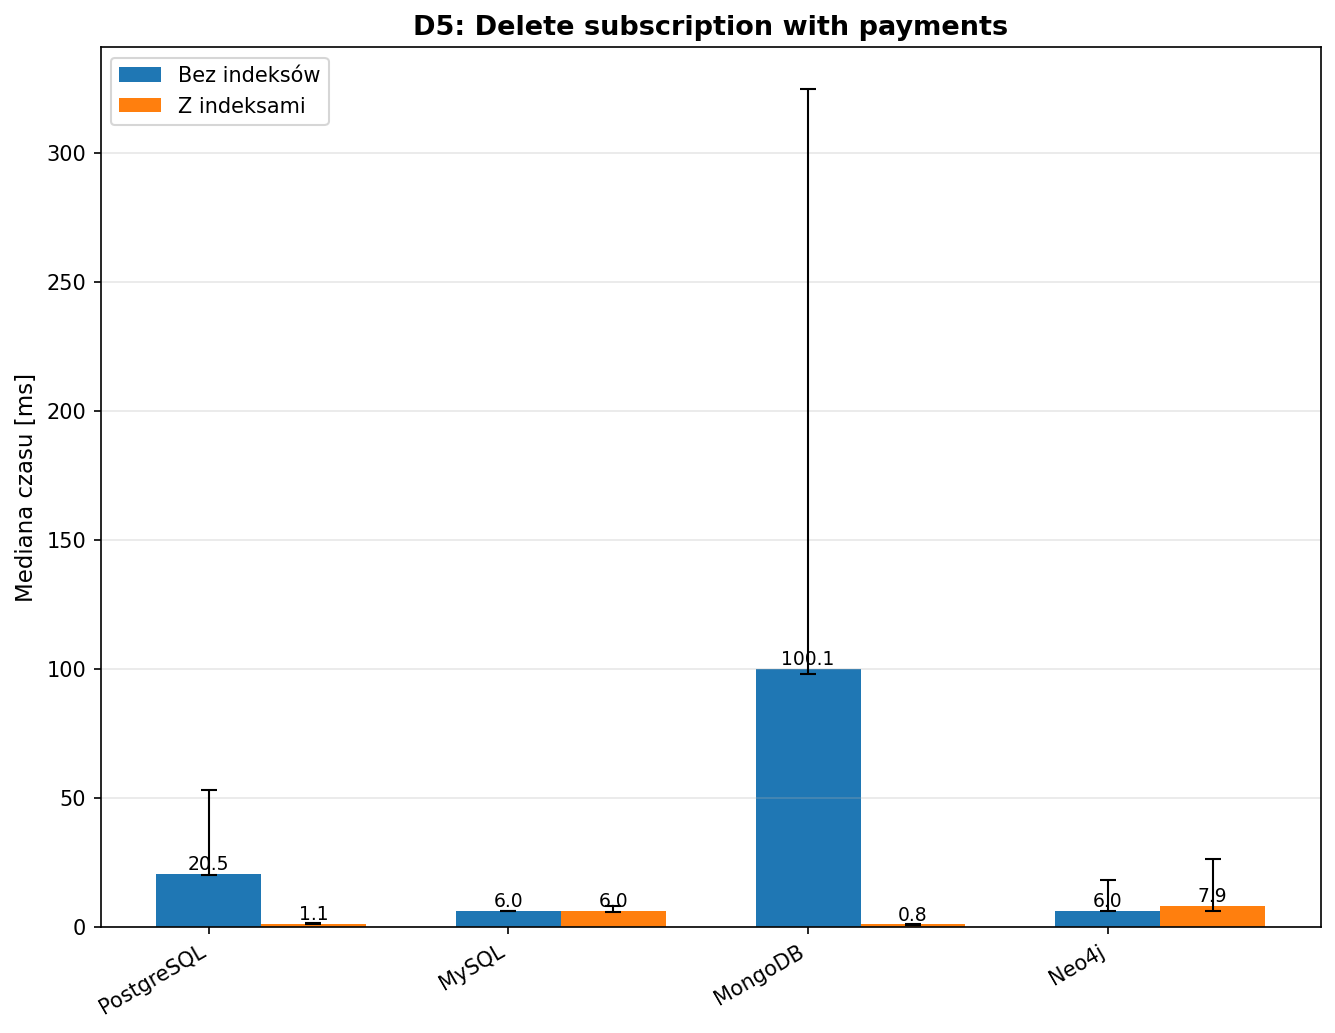
\includegraphics[width=0.8\textwidth]{charts/large/chart_D5.png}
    \caption{D5 -- Usunięcie subskrypcji z płatnościami (large)}
\end{figure}

% -------------------------------------------------------
% UPDATE
% -------------------------------------------------------

\subsubsection{U1: Aktualizacja postępu oglądania}
\begin{figure}[H]
    \centering
    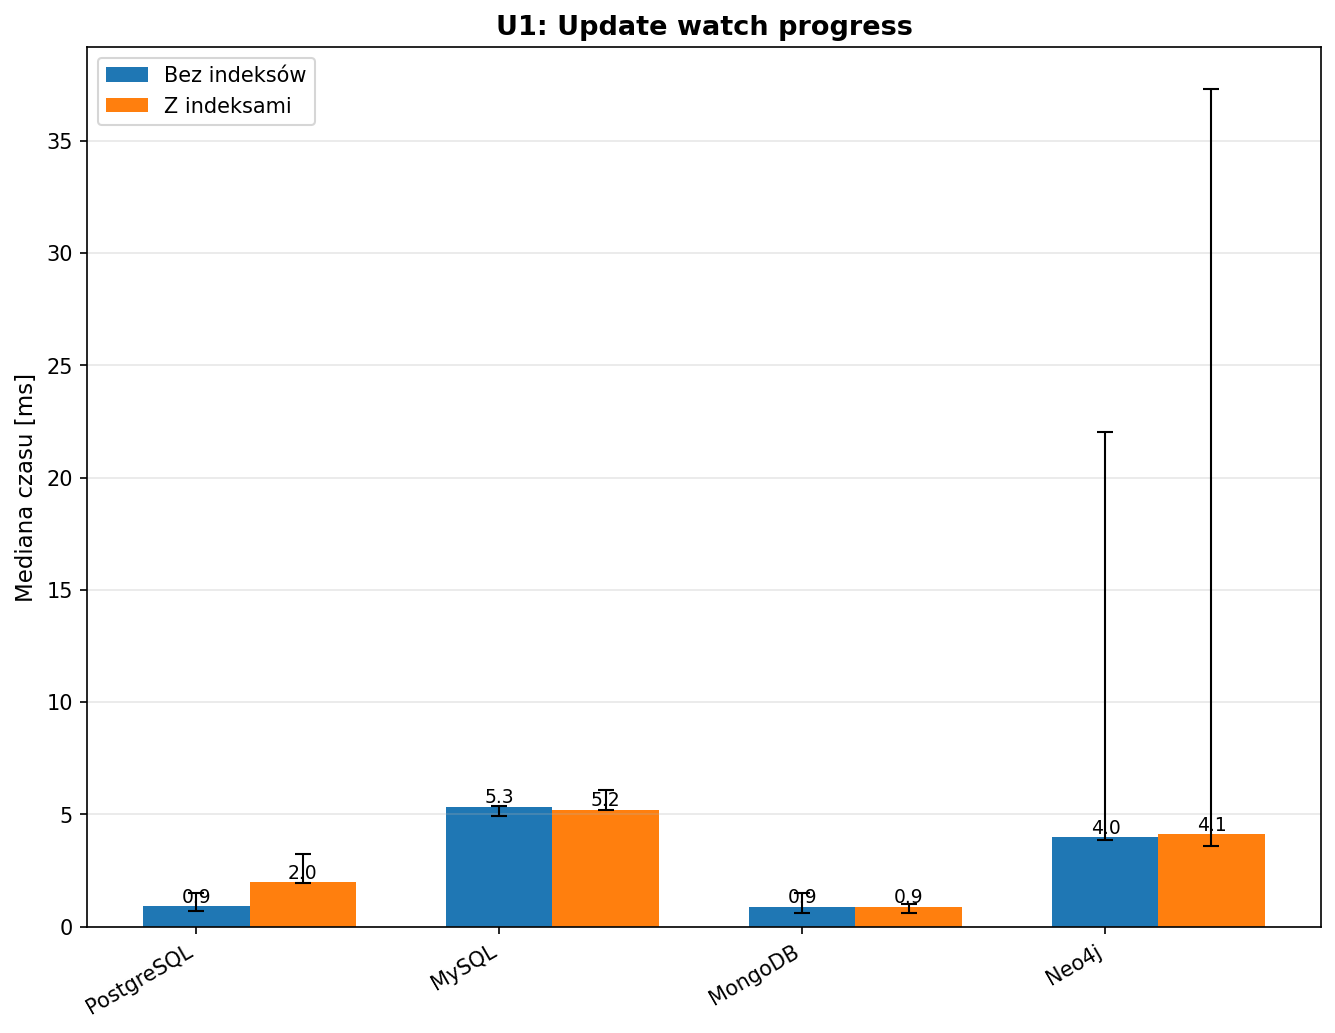
\includegraphics[width=0.8\textwidth]{charts/large/chart_U1.png}
    \caption{U1 -- Aktualizacja postępu oglądania (large)}
\end{figure}

\subsubsection{U4: Aktualizacja danych użytkownika}
\begin{figure}[H]
    \centering
    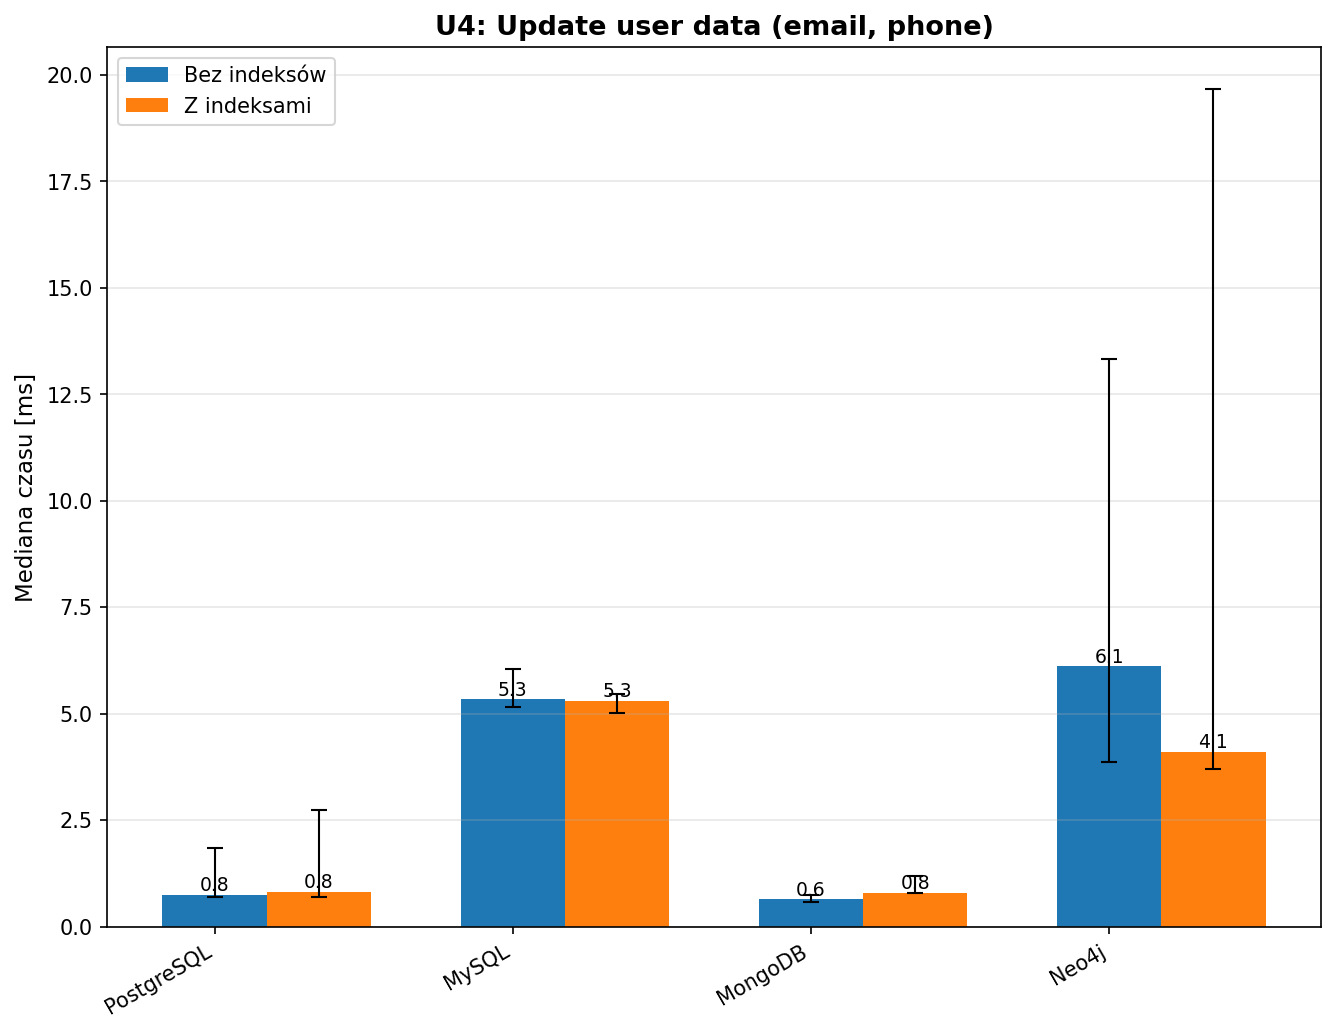
\includegraphics[width=0.8\textwidth]{charts/large/chart_U4.png}
    \caption{U4 -- Aktualizacja danych użytkownika (large)}
\end{figure}

\subsubsection{U5: Oznaczenie treści jako nieaktywnej}
\begin{figure}[H]
    \centering
    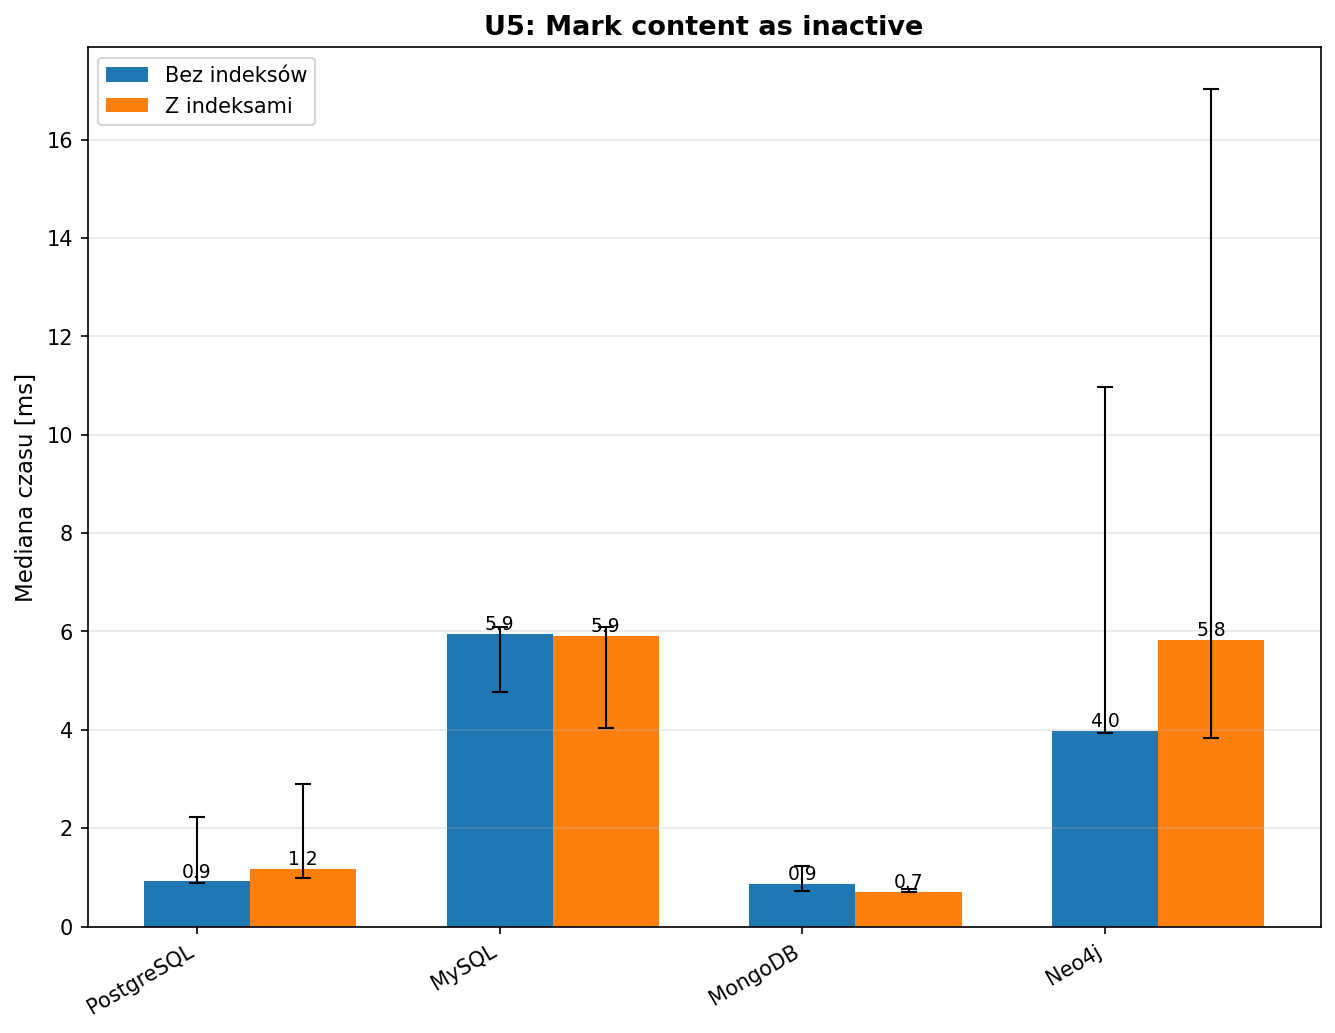
\includegraphics[width=0.8\textwidth]{charts/large/chart_U5.png}
    \caption{U5 -- Oznaczenie treści jako nieaktywnej (large)}
\end{figure}

\subsubsection{U6: Masowa aktualizacja wskaźnika popularności}
\begin{figure}[H]
    \centering
    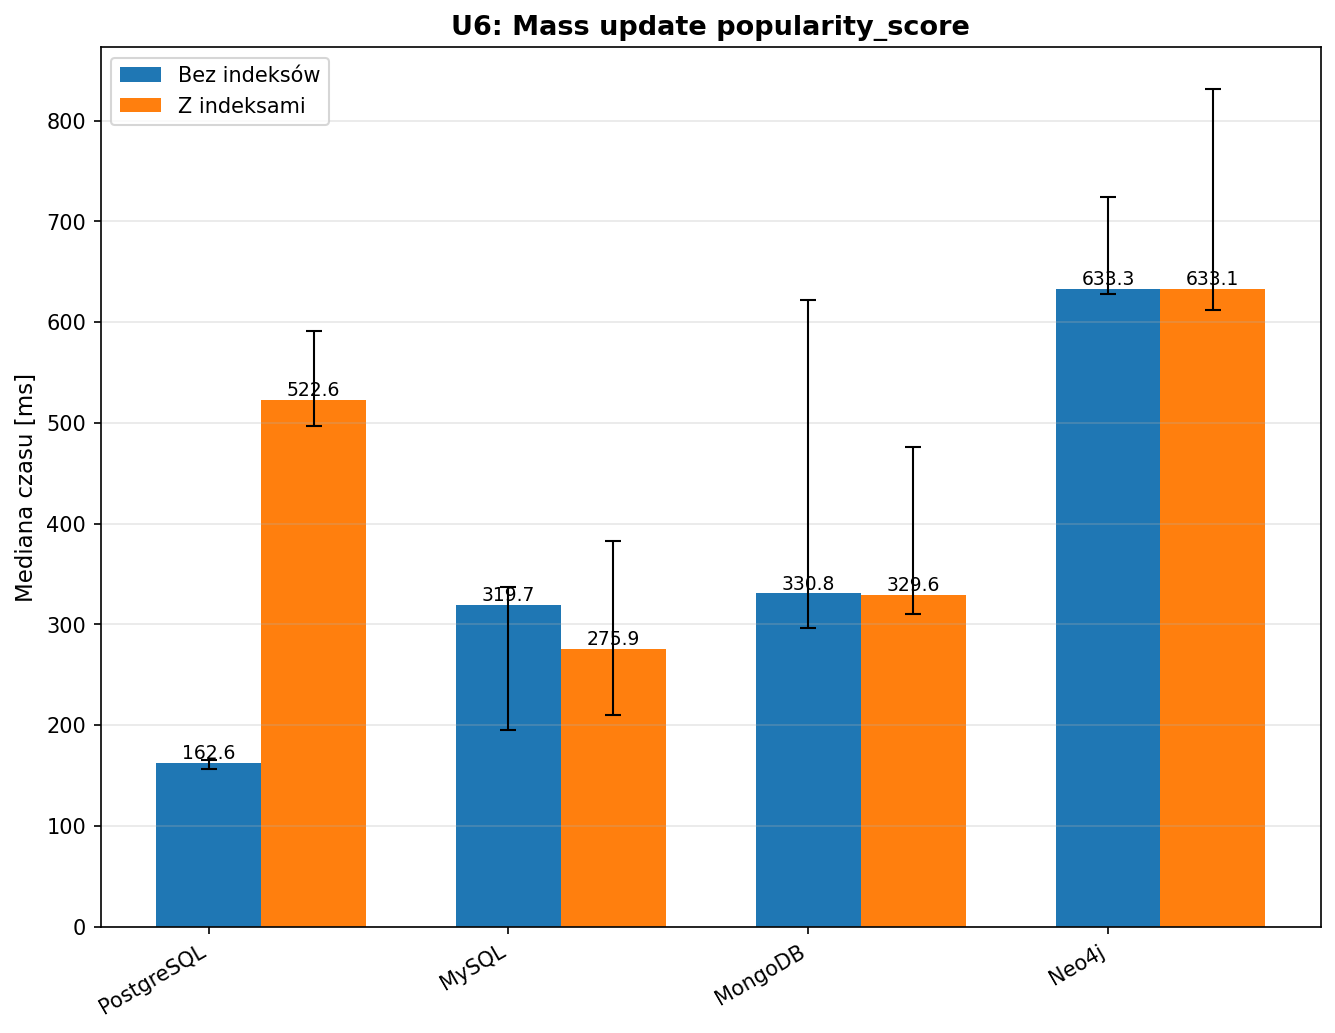
\includegraphics[width=0.8\textwidth]{charts/large/chart_U6.png}
    \caption{U6 -- Masowa aktualizacja wskaźnika popularności (large)}
\end{figure}
